% ch10: 原文 GLDraft_D.tex 行 2285–2440；§7.1–7.2
% 只译散文（标题、正文、图题、脚注）；公式、\label、\ref、\eqref、\cite、图文件名保持不变。

\section{BAA 边界条件与角的四维化身}\label{avatar}


四维超杨–米尔斯理论容许许多半 BPS 边界条件 \cite{Gaiotto:2008sa}，它们在四维 $A$-扭化中是拓扑的，并在扭化紧致化到 $C$ 上之后降为 BAA 边界条件 \cite{KW,Gaiotto:2016hvd,Gaiotto:2016wcv}。\zy{BAA 是原文沿用的一类四维半 BPS 边界条件的类型标记，本译本保留不译。关于 $\N=4$ 超杨–米尔斯理论中半 BPS 边界条件的系统分类，见 \cite{Gaiotto:2008sa}；三个字母依次标记该边界条件相对于三个复结构 $I,J,K$ 属于 A 型还是 B 型，原文未解释其读法（译者按，无外部依据）。}

这样的边界条件，连同它与 $\B_\cc$ 及 $\b\B_\cc$ 的“角”，可用来在 $\H=\Hom(\b\B_\cc,\B_\cc)$ 中定义一个量子态。我们已经用过这一构造；见图 \ref{example6}（第 \ref{wkb} 节）。除了研究更多例子之外，本节要补充的是用二维手征代数来研究这些角以及相应的量子态。

在四维中，两个边界条件之间的交汇或角出现在一个二维流形上；就我们的目的而言，这个二维流形是黎曼曲面 $C$ 的一份拷贝。对于能在四维规范场论中实现的 BAA 型膜，它与 $\B_\cc$ 的角——如果这些角同样能在四维规范场论中实现——常常是全纯-拓扑的，并支撑全纯手征代数。以此方式出现的手征代数已在 \cite{Gaiotto:2016hvd,FG} 中研究过。与 $\b\B_\cc$ 的角，如果能在四维中实现，同样通常支撑反全纯手征代数。这就是本节将要研究的情形。


\subsection{解析延拓的视角}\label{ACP}

我们首先回顾一个能简化相关交汇分析的构造。膜 $\B_\cc$ 可以从四维中的变形 Neumann 边界条件导出。\footnote{\label{deformed} 规范场的通常 Neumann 边界条件要求 $n^i F_{ij}=0$，其中 $F$ 是杨–米尔斯曲率，$n$ 是边界的法向量。变形 Neumann 边界条件则把 $n^i F_{ij}$ 用另一些场的边界值表示。注意，一个不同的、未变形的 Neumann 边界条件——它向超多重态其余部分的延拓也不同——将在第 \ref{Enriched} 节进入讨论。} 我们把它称为变形 Neumann 边界条件或 $\B_\cc$ 边界条件。

在存在这种变形 Neumann 边界时，$A$-扭化四维规范场论的路径积分，可以解释为定义在边界上的一个三维理论的一个略显奇特的路径积分 \cite{Witten:2010zr,Witten:2011zz}。这个三维理论的作用量是复变量的全纯函数，而路径积分是在场空间中的一个中间维数的积分圈（middle-dimensional integration cycle）上取的。该积分圈由四维的 $A$-模型局域化确定，但其细节对我们的目的并不重要。我们只讨论不依赖于积分圈选取的性质。我们把这类路径积分笼统地称为围道路径积分（contour path integral）。\zy{译者按（无外部依据）：“围道路径积分”（contour path integral）指把路径积分的实变量解析延拓为复变量，并沿复化场空间中的某个中间维数的圈、而不是沿整个实切片积分。关于把路径积分表示为围道积分的观点，可参见 \cite{Witten:2010zr}。}

相关的三维辅助理论，人们最熟悉的并不是它在通常几何朗兰兹中的情形，而是它在数学上所谓的“量子”几何朗兰兹中的情形。在规范场论中，这对应于在 \cite{KW} 引入的典范参数 $\Psi$ 取一般值的情形。

在一般的 $\Psi$ 下，与适当变形的 Neumann 边界条件相联系的是一个具有复联络 $\cA$ 的 Chern–Simons 理论，其曲率为 $\cF=\d \cA+\cA\wedge \cA$，作用量为
\be\label{csact} I_\CS =\frac{\Psi}{4\pi}\int_N \left( \Tr\,\cA\wedge \d \cA +\frac{2}{3}\cA^3\right). \ee
这里 $N$ 是四维流形 $M$ 的边界或边界的一部分。在 $N$ 上给出理论 $I_\CS$ 的那个边界条件是“拓扑的”，意思是定义它只需要 $N$ 的一个结构，即一个定向。若 $N=\partial M$，则 $M$ 上以“在边界上给出边界耦合 $I_\CS$”为边界条件的 $A$-模型路径积分，就是 $N$ 上一个带非标准积分圈的 Chern–Simons 路径积分（该圈依赖于 $M$）。更一般地，$N$ 本身也可以有边界；沿 $\partial N$，我们考虑给出 $I_\CS$ 的变形 Neumann 边界条件与某个别的边界条件之间的交汇或角。此时，如同带边三维流形上通常的 Chern–Simons 理论，对第二个边界条件作适当选取，沿 $\partial N$ 会出现一个流代数（current algebra）或 Kac–Moody 对称性。这些流的 level 是 $\Psi-h$，其中 $h$ 是 $G$ 的对偶 Coxeter 数（dual Coxeter number）。level 中的贡献 $\Psi$ 可以由 $I_\CS$ 在带边流形上不再规范不变这一事实经典地算出，而 $-h$ 是单圈修正，将在第 \ref{Dbc} 节描述。

就本文而言，我们关心 $\Psi=0$ 处的“通常的”几何朗兰兹。若简单地在作用量 (\ref{csact}) 中令 $\Psi=0$，我们得不到任何有意义的东西，因为作用量为零的围道路径积分没有意义；事实上，不存在既取极限 $\Psi\to 0$ 又保持沿 $N$ 的拓扑不变性的办法。这是理解下述事实的一种方式：本文中一直很重要的 $\B_\cc$ 边界条件是全纯-拓扑的，而不是拓扑的。为取 $\Psi\to 0$ 的极限以得到全纯-拓扑边界条件，可以这样做。设 $C$ 是带局部复坐标 $z$ 的复黎曼曲面，并设 $N=S\times C$，其中 $S$ 是由 $t$ 参数化的一维流形。然后取极限 $\Psi\to 0$，同时保持 $\varphi=\frac{\Psi}{4\pi} \cA_z\d z$ 固定。Chern–Simons 作用量变为
\be\label{degac}
I_{\varphi\cF}= 
\int _N\Tr\, \varphi_z \cF_{t \bar z} \d t \d^2z.
\ee

Chern–Simons 作用量 (\ref{csact}) 退化为式 (\ref{degac}) 的作用量，这与随着希格斯丛模空间 $\M_H(G,C)$ 的复结构变动、复平坦联络退化为希格斯丛有些类似。作用量 $I_{\varphi\cF} $ 所描述的东西，可以解释为 $C$ 上 $(0,1)$ 联络空间的余切丛上的拓扑规范量子力学。希格斯场 $\varphi$ 是 $\cA_{\bar z}$ 的共轭动量。用二维语言说，类似的说法是：带 $\B_\cc$ 边界的 $\M_H(G,C)$ 的 $A$-模型，与 $\M_H(G,C)$ 上一个解析延拓的量子力学有关 \cite{Witten:2010zr}。

这一表述使下述事实变得显然：变形 Neumann 边界条件在 $A$-扭化中不是拓扑的。相反，它依赖于 $C$ 上复结构的选取，并容许沿 $C$ 全纯变化、沿 $S$ 拓扑变化的局部算符：它是一个全纯-拓扑边界条件。由 $I_{\varphi\cF}$ 导出的运动方程蕴含 $\varphi$ 关于 $z$ 全纯且与 $t$ 无关。在远离 $N$ 的边界处，$N$ 上的规范不变局部算符是 $\varphi$ 的规范不变多项式 ${\cal P}[\varphi](z)$——它们在二维 $A$-模型中降为 Hitchin 哈密顿量——以及这些算符的费米子伴（fermionic partners），后者在附录 \ref{coho} 中描述。（在一般的 $\Psi$ 下，以 Chern–Simons 作用量 $I_\CS$ 刻画的边界上没有规范不变局部算符。）

若 $N$ 有边界，会发生什么？给出 $\varphi\cF$ 理论的变形 Neumann 边界条件与一个拓扑的四维边界条件之间的交汇，在许多情形下可以用 $\varphi\cF$ 理论中的一个边界条件来描述，后者同时编码该拓扑边界条件与交汇的选取。在许多重要的例子中，该拓扑边界条件是 BAA 型的半 BPS 边界条件。在适当的选取下（我们将在第 \ref{Dbc} 节进一步讨论），$\varphi$ 沿 $\partial N$ 的行为可以像一个生成 Kac–Moody 对称性的全纯流。但现在 Kac–Moody 对称性的 level 完全来自单圈修正，等于 $-h$。

一般而言，出现在 $\varphi\cF$ 辅助规范场论中的边界条件也是全纯的，并可能支撑全纯局部算符。这反映了变形 Neumann 边界与半 BPS 边界之间相应交汇的同一性质：它们在 $A$-扭化理论中是全纯的。\zy{译者按（无外部依据，据原文校勘）：原文此处作 “deformed Neuman boundary”，脱去一个 n，当为 “deformed Neumann boundary”（变形 Neumann 边界条件）；本节前文即作 Neumann。译文按 Neumann 处理，特此说明。} 一般 $\Psi$ 下 GL 扭化理论中全纯交汇的出现及其与 Chern–Simons level 的关系，已在 \cite{Gaiotto:2017euk} 中分析。

\subsection{手征代数的作用} \label{RoleChiral}
全纯-拓扑边界条件与拓扑边界条件之间的全纯交汇，可能支撑全纯依赖于其在 $C$ 上位置的局部算符。本质上按定义，这些算符定义一个手征代数。尽管该手征代数同时依赖于拓扑边界条件的选取和交汇的选取，为记号简便我们将略去这种依赖，直接把手征代数记作 ${\cal V}$。这个手征代数类似于二维共形场论中、或三维拓扑场论（TFT，如 Chern–Simons 理论）边界处所能找到的全纯局部算符的手征代数。由于 $\varphi \cF$ 理论是全纯-拓扑的，这里存在一些差别 \cite{Costello:2020ndc}。

在 $A$-扭化理论中，单个交汇可用来在二维 $A$-模型中构造各种不同的角，具体取决于放置在 $C$ 中点 $z_i$ 处的局部算符 $O_i(z_i)$ 的选取。这些角并不全都彼此独立：它们全纯地依赖于 $z_i$，而 $z_i \to z_j$ 时的奇异性由手征代数的 OPE 控制。OPE 或相应的 Ward 恒等式蕴含不同角之间的递推关系。\footnote{手征代数的 Ward 恒等式的解通常称为{\it 共形块}（conformal block）。在物理的二维共形场论中，共形块通常可以通过黎曼曲面上的某种缝合手续得到。对 ${\cal V}$ 这样的一般手征代数，这未必可行，但共形块的概念仍然可用，并可用于刻画由给定交汇所能产生的 $A$-模型角的空间。}

回顾变形 Neumann 边界条件上那些给出 Hitchin 哈密顿量的规范不变局部算符 ${\cal P}[\varphi](z)$。这些算符可以沿边界上的拓扑方向 $t$ 移到交汇处。由此得到的“边界到交汇”OPE 不是奇异的，并产生 ${\cal V}$ 中的一族算符 $S_{\cal P}(z)$。这些算符是{\it 中心的}（central），即它们与 ${\cal V}$ 中其他算符的 OPE 非奇异；理由与 ${\cal P}[\varphi](z)$ 彼此 OPE 非奇异相同：它们可以沿 $t$ 方向自由移动。

这一性质有一个重要的推论：以一族算符 $S_{\cal P}(z) O_1(z_1) \cdots O_n(z_n)$ 标记的 $A$-模型角，作为 $z_i$ 的函数满足与仅以 $O_1(z_1) \cdots O_n(z_n)$ 标记的角相同的 Ward 恒等式。这就保证了 ${\cal P}[\varphi](z)$ 在这个 $A$-模型角空间上的作用是良定义的。\zy{原文此句作 “This insures that the the action”，多出一个 “the”；本节后文（关于 't Hooft 算符处）同一句又出现一次。中文无法体现，特此说明。}


 \begin{figure}
 \begin{center}
   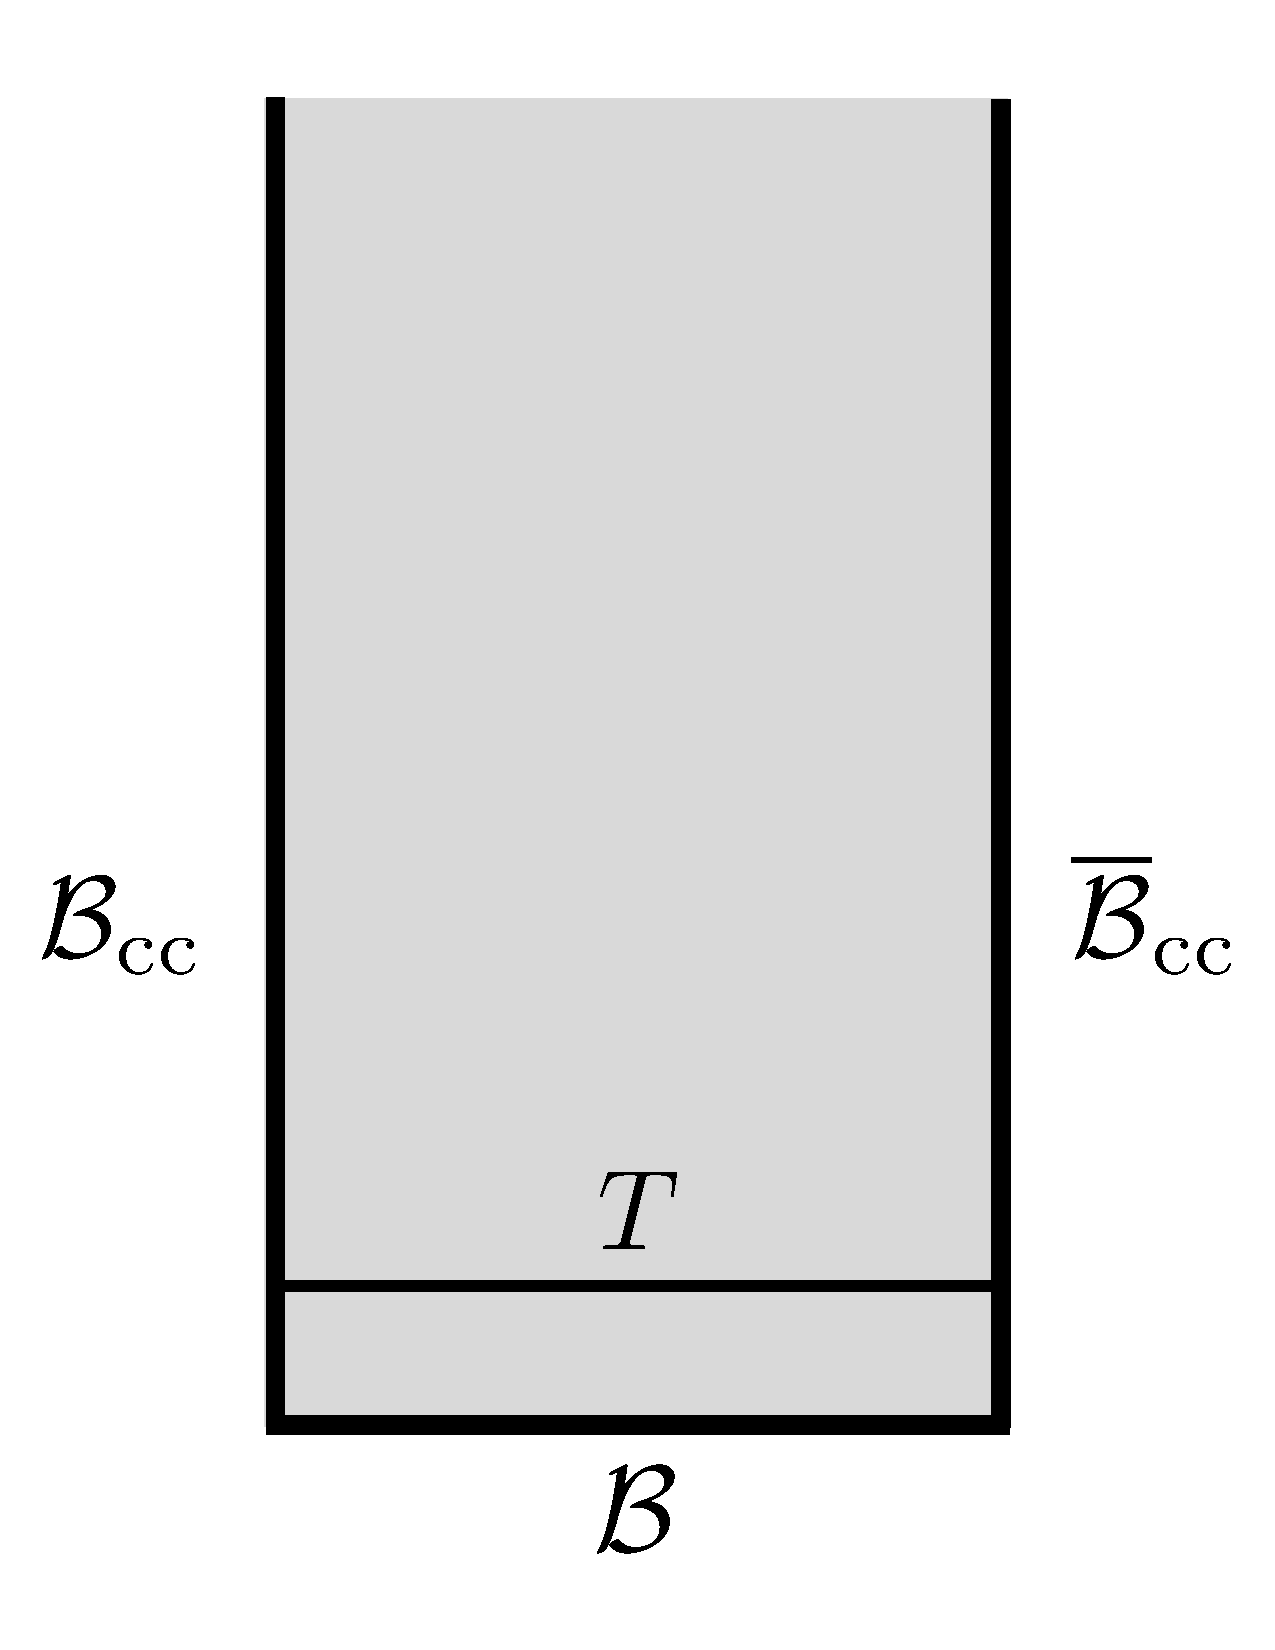
\includegraphics[width=1.7in]{Example8.pdf}
 \end{center}
\caption{\small 一个 BAA 型的 't Hooft 算符 $T$，作用在由 BAA 型膜 $\B$ 生成的态上，并附有适当的手征角。我们可以把 $T$ 与 $\B$ 融合，得到一个新的 BAA 型膜 $T\B$。这涉及我们在图 \ref{example1}(a) 中最初讨论的线算符对膜的作用。此外，我们还须考虑 $T$ 与 $\B$ 的左、右端点或边界处各手征角的复合。  \label{example8}}
\end{figure} 

我们也可以讨论：在用手征代数角描述 't Hooft 算符对膜所生成的态的作用的四维图景中，会出现哪些手征代数要素。在图 \ref{example8} 中，我们勾勒了一个 BAA 型的 't Hooft 算符 $T$，它作用在由同型膜 $\B$ 生成的态上，并带有适当的手征角与反手征角。$T$ 对态的作用可以描述为：把 $T$ 所代表的界面与边界 $\B$ 融合，同时把相应的角分别与 $\B_\cc$ 及 $\bar \B_\cc$ 作复合。在四维中，与图 \ref{example8} 的二维图像不同，'t Hooft 线缺陷与半 BPS 边界之间有明显的差别：前者支撑在一点 $p\in C$ 处，而后者缠绕整个 $C$。所以复合 $T\B$ 在远离 $p$ 处与 $\B$ 重合；它可以描述为用一条线缺陷增广的膜 $\B$。因此，为描述 't Hooft 算符的作用，我们首先应当把本节的讨论推广到允许边界线缺陷在一点 $p\in C$ 处终结于交汇的情形。照例，这一设置将全纯地依赖于 $p$。它之所以只依赖于 $p$，是因为在 $A$-扭化理论中，边界线缺陷本身是一个拓扑 't Hooft 线缺陷的像，因而也是拓扑的。

边界线缺陷 $\ell$ 及其端点的存在，既不影响 $C$ 上其他位置可用的手征代数算符的选取，也不影响它们在远离 $p$ 处满足的 Ward 恒等式。但它影响它们在 $p$ 附近的行为。对每个 $\ell$，可能的端点 $O_{\ell,i}(p)$ 构成一个向量空间，而它们构成 ${\cal V}$ 的一个模 ${\cal V}_\ell$：模结构编码手征代数算符与端点之间的 OPE，并控制在 $p$ 处由 ${\cal V}_\ell$ 的插入所满足的 Ward 恒等式。

当我们把一个端点为 $\alpha_{R,n}(p)$ 的 't Hooft 算符移到半 BPS 边界处时，会产生一条边界缺陷 $\ell$，同时在交汇处产生一个特定的端点 $S_{R,n}(p) \in {\cal V}_\ell$。我们可以预言这类端点的两个一般性质：它们与手征代数 ${\cal V}$ 的 OPE 非奇异，就像与 Hitchin 哈密顿量相关联的 $S_{\cal P}(z)$ 那样；并且它们满足与 $\alpha_{R,n}(p)$ 相同的关于 $p$ 的微分方程，其系数由 $S_{\cal P}(z)$ 控制。这些性质可以立即导出：沿拓扑方向把 't Hooft 线与边界分开，再把 $S_{R,n}(p)$ 变回 $\alpha_{R,n}(p)$ 即可。

同样，中心性保证：以一族算符 $S_{R,n}(p) O_1(z_1) \cdots O_n(z_n)$ 标记的 $A$-模型角，作为 $z_i$ 的函数满足与仅以 $O_1(z_1) \cdots O_n(z_n)$ 标记的角相同的 Ward 恒等式。这就保证了 't Hooft 算符对膜所生成的态的作用是良定义的。

我们以关于辅助 $\varphi F$ 理论中 't Hooft 线描述的几点评论来结束这一一般性讨论。垂直于 $N$ 的 't Hooft 线可以解释为 $\varphi F$ 理论中的单极子局部算符。${\cal P}[\varphi](z)$ 这样的算符同时作为 $\varphi F$ 理论和四维理论中的局部算符出现，因为它们是基本场的多项式，其定义不依赖于路径积分围道的选取。相反，单极子算符这类无序算符的定义，要求修改路径积分所允许的场构型空间，从而影响积分围道的可能选取。这种修改体现为：四维理论中实际存在一条线缺陷，它在 $N$ 中的 $p$ 处终结。这些考虑也适用于 $\partial N$ 处的边界无序算符；它们将表现为四维理论中一条边界线缺陷的端点 $O_{\ell,i}(p)$。

直接分析 $\varphi F$ 理论中可用的单极子算符空间以及它们在边界处的像，将会很有意义。其中的一些工具已在 \cite{Gaiotto:2016wcv} 中发展出来，并在那里应用于 Chern–Simons 理论。它们涉及仿射 Grassmann 流形上的上同调计算，这些计算很可能给出第 \ref{lineq} 节分析的局部版本。我们把这个练习留给热心的读者。\zy{译者按（无外部依据，据原文校勘）：原文此处作 “affine Grassmanian”，系 “affine Grassmannian”（仿射 Grassmann 流形）之误；本译本按后者处理。}

